\section{Image processing}\label{sec_image_processing}
The purpose of this section is to identify the location housing part in a image. This is done in two parts, firstly by detecting the blob in the image and secondly calculating the centroid of the blob.

\subsection{Blob detection}\label{sub_blob_detection}
A single frame from the camera in the test setup is shown on figure \ref{fig_clean_pic}.
\begin{figure}[htpb!]
	\centering
\begin{tikzpicture}
\node[anchor=south west,inner sep=0] (image) at (0,0) 
{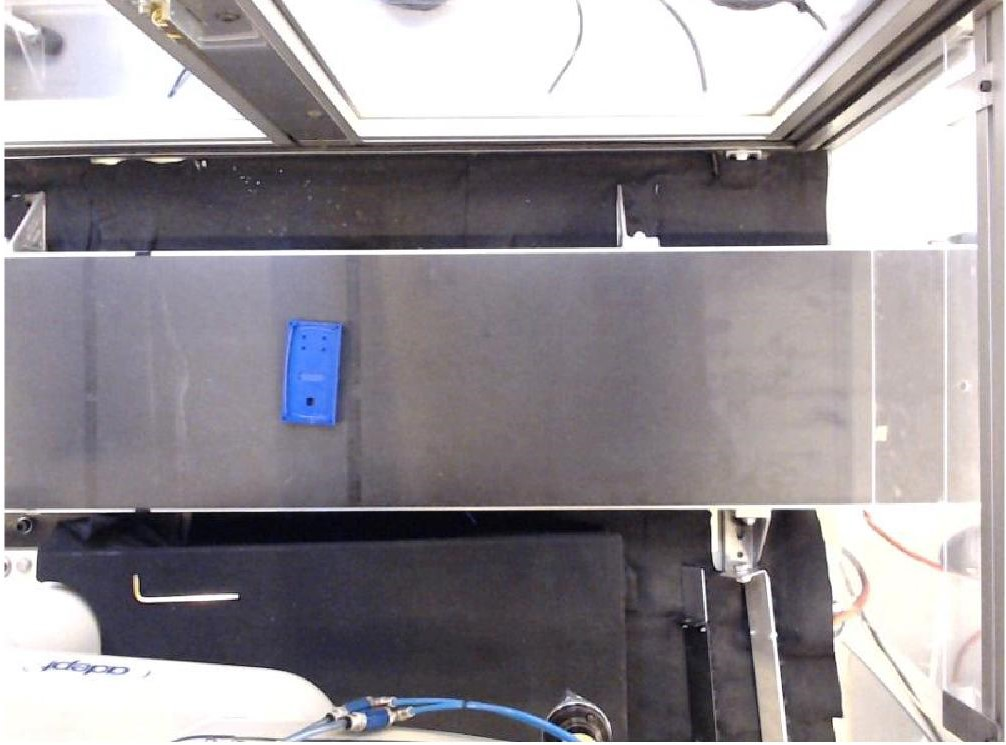
\includegraphics[width=0.6\textwidth]{clean_pic}};
		\begin{scope}[x={(image.south east)},y={(image.north west)}]
	   		\draw[very thick,red] (0.095,0.375) --(0.095,0.657) --node[above,red]{Region of interest} (0.79,0.665)  -- (0.79,0.382) -- (0.095,0.375);
	    \end{scope}
	\end{tikzpicture}
	
	\caption{A single image from the camera in the test setup}
	\label{fig_clean_pic}
\end{figure}\newline
First step is to define the region of interest, which is shown on the figure. This is done by defining the determining the pixels spanning this region, and creating a new image containing all the pixels within the region of interest. The resulting image is shown on figure \ref{fig_roi}.
\begin{figure}[htbp]
	\centering
	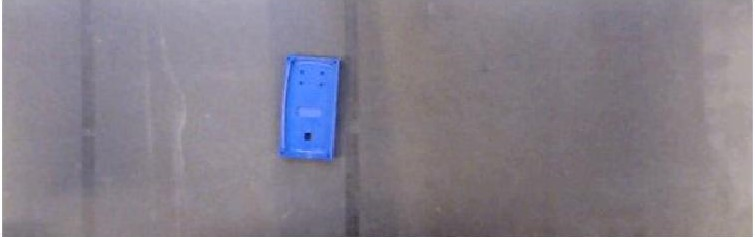
\includegraphics[width=0.8\textwidth]{roi_pic}
	\caption{The region of interest, which is the conveyor belt}
	\label{fig_roi}
\end{figure}  \\
With the new image only showing the housing part and conveyor belt, the next step is the algorithm needs to determine the difference between these two. The first attempt is background subtraction, the idea is, that if the background is static, then by subtracting it from the image, only the housing will remain. A base picture of the background is shown on figure \ref{fig_base}.
\begin{figure}[htbp]
	\centering
	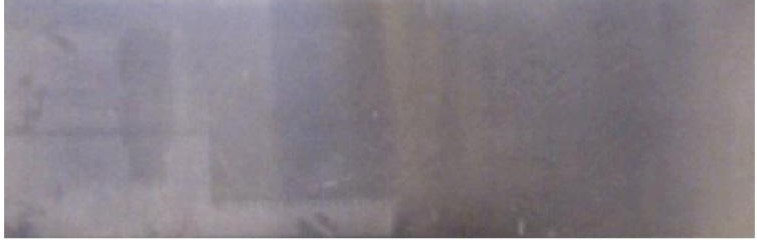
\includegraphics[width=0.8\textwidth]{base_pic}
	\caption{The base image, which only shows the conveyor belt}
	\label{fig_base}
\end{figure}  \\
Comparing this base image with figure \ref{fig_roi}, a conflict with the assumption about static background arises. The conveyor belt's appearance is not uniform and there are tape lines from previously experiments, these might cause noise later in the vision algorithm. Before the subtraction it is decided to work with greyscale images, so where the frame and base currently are in the RGB space, this is done with a weighted summation
\begin{align}
f(u,v)=\alpha\g R+\beta\g G+\gamma \g B\\
\alpha+\beta+\gamma=1
\end{align}
In this first attemp $\alpha=1$ and $\beta=\gamma=0$. The background subtraction is done with the following equation:
\begin{equation}
g(u,v) = |f(u,v)-b(u,v)|
\end{equation} 
Where $u$ is the pixel number in the vertical direction, $v$ the pixel number in the horizontal direction, $f$ is the actual frame and $b$ is the base image, the absolute value is used, since it is likely some pixels' value might become negative and negative pixel values does not correspond to a nuance of grey. Figure \ref{fig_sub} shows the result of subtracting the base image from figure \ref{fig_roi}.\clearpage
\begin{figure}[htbp!]
	\centering
	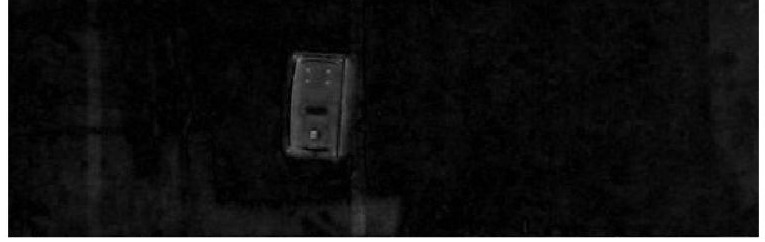
\includegraphics[width=0.8\textwidth]{background_pic}
	\caption{The resulting image after the base is subtracted from the frame}
	\label{fig_sub}
\end{figure} 
\noindent The background subtraction did not manage to remove the entire background, which results in some additional grey areas in the frame besides where the housing is located.  Next step is to try and remove these additional grey areas which is acting a noise in the frame. This is done by performing thresholding on the frame, which transform it from greyscale form into binary form. To determine which thresholding value to use, it is necessary to make a histogram for figure \ref{fig_sub}. The appropriate thresholding value is a compromise between false positive and false negatives, meaning backgrounds pixels which are set to 1 and pixels belonging to the housing set to 0. The histogram is shown on figure \ref{fig_histo_grey}.
\begin{figure}[htbp!]
	\centering
	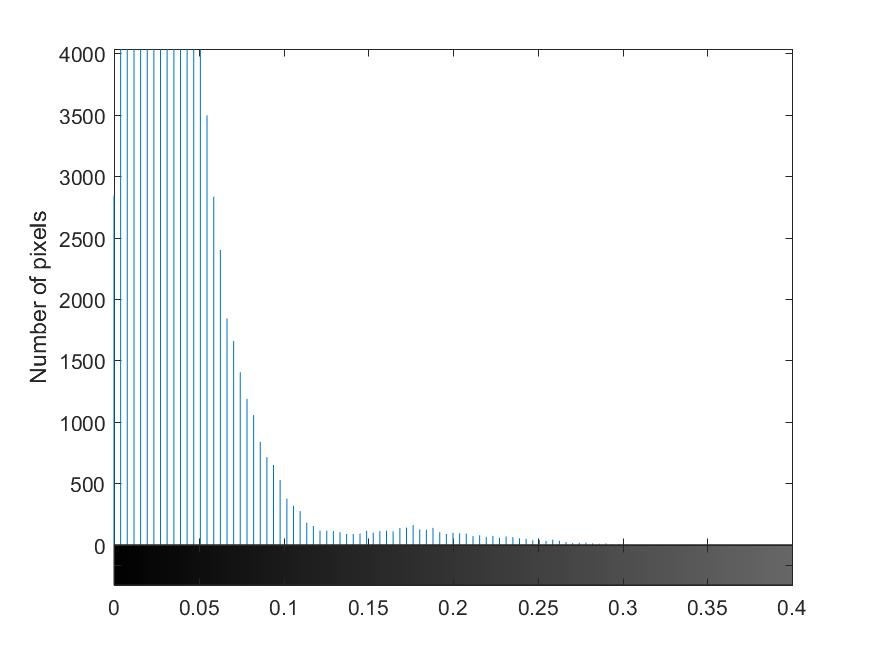
\includegraphics[width=0.8\textwidth]{histo_pic}
	\caption{Histogram for the frame in figure \ref{fig_sub}}
	\label{fig_histo_grey}
\end{figure}\\
The leftmost part of the histogram is the background, so a candidate thresholding value is $t=0.15$. The logic used for creating the resulting binary frame is:
\begin{equation}
T = \left\{\begin{matrix}
g(u,v)\geq t \rightarrow T(u,v)=1\\[1em]
g(u,v)<t \rightarrow T(u,v)=0
\end{matrix}    \right.
\end{equation}\clearpage
Doing this for the entire frame yields the binary frame shown on figure \ref{fig_binary_v1}
\begin{figure}[htbp]
	\centering
	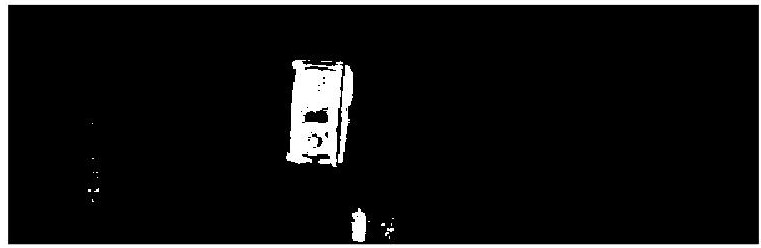
\includegraphics[width=0.8\textwidth]{tresh_static}
	\caption{The resulting binary frame}
	\label{fig_binary_v1}
\end{figure}
A blob is defined as a connected white area, but the problem here is, the blob generated by the housing is deformed and broken. Following the same approach for different frames, shows that the blob is always deformed and broken, so it is necessary to use a different method for blob detection.
\subsubsection{HSI colorspace}
In the book \citep{image} it is proposed to use the HSI color space for video, since it is feasible to assume that the housing color is unique throughout the video sequence. The acronym HSI stands for; Hou, Saturation and  intensity.  Hou is the pure color, Saturation is the amount of white light mixed with the Hou color. Lastly the Intensity is calculated as. \citep{image}
\begin{equation}
I=\frac{R+G+B}{3},~~I\in[0,255]
\end{equation} 
The two remaining are calculated from the RGB color space as such: \citep{image}
\begin{align}
	H &= \left\{\begin{matrix}
		cos^{-1}\left(\frac{1}{2} \frac{(R-G)+(R-B)}{\sqrt{(R-G)(R-G)+(R-B)(G-B)}}\right),~G\geq B\\
		360^o-cos^{-1}\left( \frac{1}{2}\frac{(R-G)+(R-B)}{\sqrt{(R-G)(R-G)+(R-B)(G-B)}}\right),~G<B
	\end{matrix}   \right.,~~H\in[0,360[\\[0.5em]
	S &=1-3\g\frac{\min\{R,G,B\}}{R+G+B},~~S\in[0,1]
	\end{align}
Doing this for the frame in figure \ref{fig_roi} yields the new frame which is shown on figure \ref{fig_hsi}.
\begin{figure}[htbp!]
	\centering
	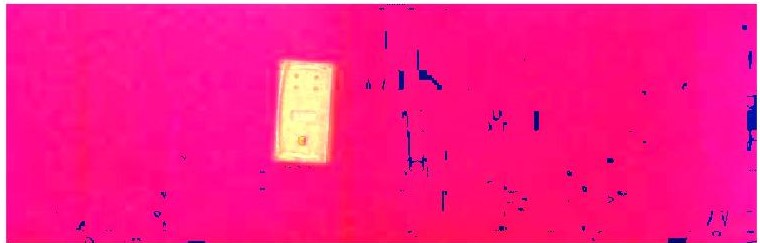
\includegraphics[width=0.8\textwidth]{HSI_pic}
	\caption{The frame converted into the HSI color space}
	\label{fig_hsi}
\end{figure}\\
There is a clear distinction between the housing and the conveyor belt, the most notable difference is the vertical lines on the conveyor, which caused noise before, are not viseable in the HSI frame. It is also possible to do background subtraction on the HSI frame, but to begin with, the thresholding is done on the Hou and Saturation values. The histogram for these two are shown on figure \ref{fig_hsi_histo}.
\begin{figure}[htbp!]
	\centering
	\begin{subfigure}[t]{0.45\textwidth}
		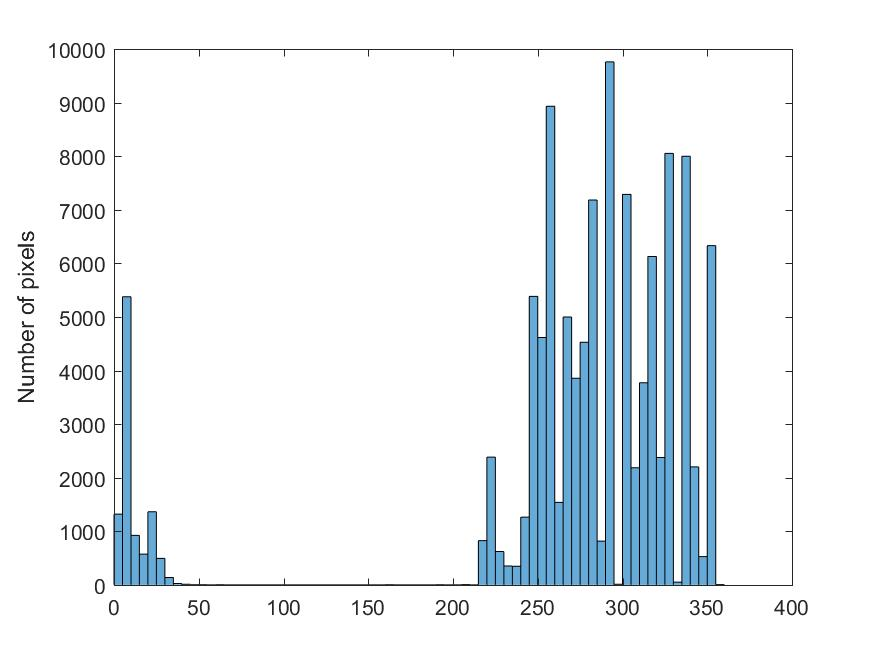
\includegraphics[width=\textwidth]{histo_H}
		\caption{Histogram for the Hou values in the HSI frame}
		\label{fig_histo_h}
		\end{subfigure}~~
	\begin{subfigure}[t]{0.45\textwidth}
		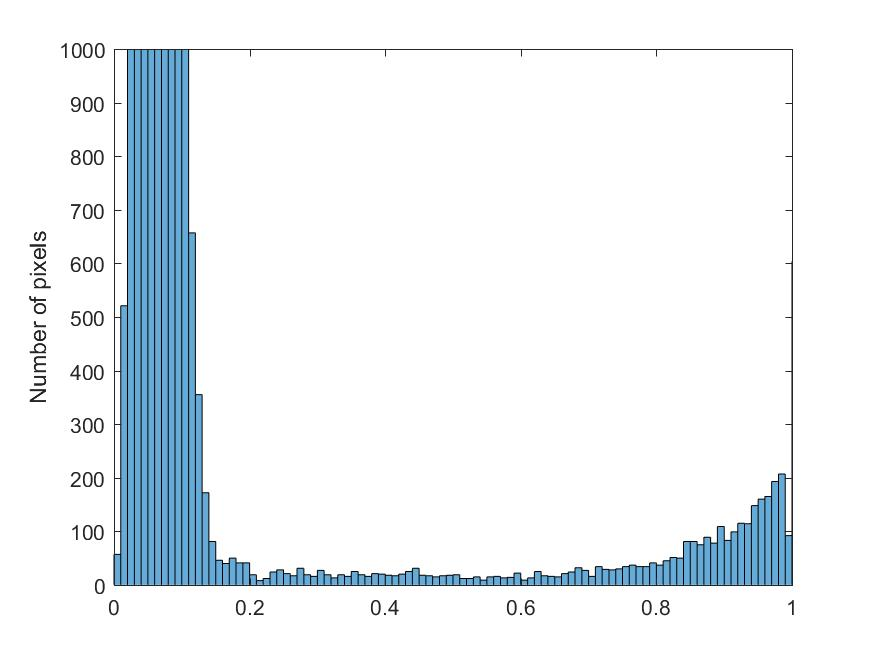
\includegraphics[width=\textwidth]{histo_S}
\caption{Histogram for the Saturation values in the HSI frame}
\label{fig_histo_s}	
	\end{subfigure}
\caption{}
\label{fig_hsi_histo}
\end{figure} \\
By probing the pixel values on figure \ref{fig_hsi} it is possible to determine the range for the Hou and Saturation values, which are as follows:
\begin{align}
H&\in[180,250]\\
S&\in[0.4,1]	
\end{align}
The programming used for thresholding is:
\begin{lstlisting}
for i = 1:ilg
	for j = 1:ihg
		if (HSI(i,j,1) >= 180 && HSI(i,j,1) <= 230  
		    && HSI(i,j,2) >= 0.4 && HSI(i,j,2) <= 1)
			g(i,j) = 1;
		else 
			g(i,j) = 0;
		end
	end
end
\end{lstlisting}
Where $ilg$ and $ihg$ is respectively the height and width of the frame in pixels. As before this thresholding yields a binary image, which is shown on figure \ref{fig_bin_hsi}. \clearpage
\begin{figure}[htbp!]
	\centering
	
\includegraphics[width=0.8\textwidth]{thres_hsi}
	\caption{The resulting binary frame after thresholding the HSI frame}
	\label{fig_bin_hsi}
\end{figure}
\noindent There is some small holes in the blob but all the background is removed and the blob is deemed a adequate representation of the housing. 
\subsection{Determination of centre and orientation}
The purpose is to determine position and orientation of the housing such that the robot can place a lid correctly on it. The way this is done to begin with by the vision system, is to determine the centroid of the blob found in the previous section and afterwards it is possible to find the orientation. The first step is to determine the size of the blob and number of blobs in the frame, this is done by comparing a pixel to its' neighbours. If the neighbours are white pixels they are connected and if they are black, they are not. Thereby it is possible to set up a book keeping matrix of the same size as the frame which keeps track of which pixels are background and which pixels belongs to a given blob. This is all handled by the MATLAB command: \citep{vision}
\begin{lstlisting}
blob = iblobs(g,'area',[min max])
\end{lstlisting}    
This command takes the binary frame and only returns the blobs which areas are within the limits, the area is defined as the number of pixels within the blob. Once the blob is known it is necessary to determine the bounding box, this is the smallest possible box which still fully contain the blob. Firstly it is necessary to determine the maximum and minimum non-zero pixel in both the u- and v-direction within the blob, since these will form the corners of the box.  The result of this is shown on figure \ref{fig_bound_box}, where the box derived from the binary frame is plotted on top of the frame from the camera. \citep{vision}
\begin{figure}[htbp!]
	\centering
	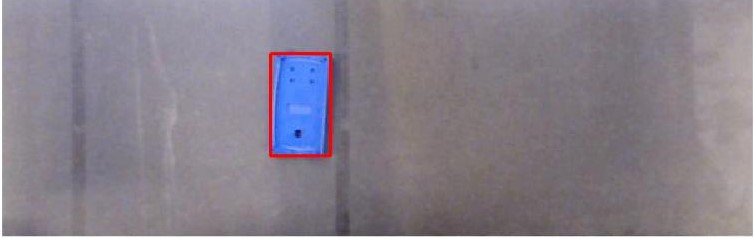
\includegraphics[width=0.8\textwidth]{box_hsi}
	\caption{The frame from the camera where the bounding box is laid on top}
	\label{fig_bound_box}
\end{figure}\\
As expected the box fully contains the housing, which verifies the quality of the binary frame. The next step is to calculate the center of the blob, this is done using the image moment. If the all the pixels within the housing blob and only these is said to be contained in the new frame $H(u,v)$, which is the same size as the binary frame, then the moment for $H$ is defined as: \citep{vision}
\begin{equation}
m_{qp}=\sum_{(u,v)\in H} u^p\g v^q\g H(u,v)
\end{equation} 
The sum $(p+q)$ is the order of the moment, where the zero order moment is defined as
\begin{equation}
m_{00}=\sum_{(u,v)\in H}H(u,i)
\end{equation}
A physical interpretation of the moments, is mass distribution where the pixels represent units of area and mass. With this in mind it is possible to calculate the centre of mass or more commonly within vision, the centroid of the region as:
\begin{align}
u_c&=\frac{m_{10}}{m_{0}}\\[0.5em]
v_c&=\frac{m_{01}}{m_{00}}
\end{align}  
Adding this centroid to the previous plot yields the result shown on figure \ref{fig_cent}
\begin{figure}[htpb!]
	\centering
	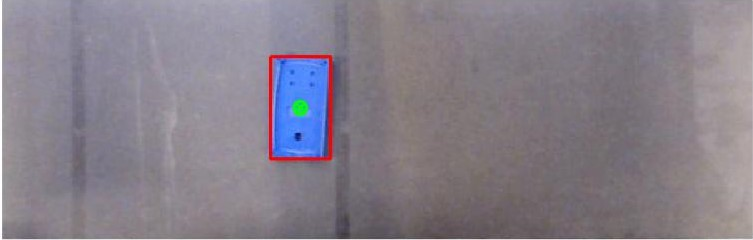
\includegraphics[width=0.8\textwidth]{cent_hsi}
	\caption{The frame from the camera with the bounding box and the centroid plotted}
	\label{fig_cent}
\end{figure}
Lastly to calculate the orientation of blob, this is done by introducing the central moments $\mu_{pq}$ defined as:
\begin{equation}
\mu_{pq}=\sum_{(u,v)\in H} (u-u_c)^p(v-v_c)^qH(u,v)
\end{equation}
The central moments are invariant with respect to position and relate to the moments in the following way:
\begin{align}
\mu_{10}&=0\\
\mu_{01}&=0\\
\mu_{20}&=m_{20}-\frac{m_{10}^2}{m_{00}}\\
\mu_{02}&=m_{02}-\frac{m_{01}^2}{m_{00}}\\
\mu_{11}&=m_{11}-\frac{m_{01}\g m_{01}}{m_{00}}
\end{align}
Giving these central moments a physical interpretation, as before, they describe the inertia of the blob and can be inserted in a inertia matrix.
\begin{equation}
J=\mat{\mu_{20} & \mu_{11}\\\mu_{11} & \mu_{02}}
\end{equation}  
The orientation is calculated by finding a equivalent ellipse which has the same inertia matrix as $H$, this is done by using the  eigenvectors of the inertia matrix. The eigenvectors gives the ellipses' principal axes. The major axis, $v_y$, correspond to the eigenvector associated to the largest eigenvalue of the inertia matrix and likewise the minor axis, $v_x$, is given by the eigenvector associated with the smallest eigenvalue. Thereby the orientation with respect to the horizontal axis is given by:
\begin{equation}
\theta = \tan^{-1}\left(\frac{v_y}{v_x}\right)
\end{equation}   
The equivalent ellipse is added to the frame from the camera on figure \ref{fig_ellipse}.
\begin{figure}[htbp!]
	\centering
	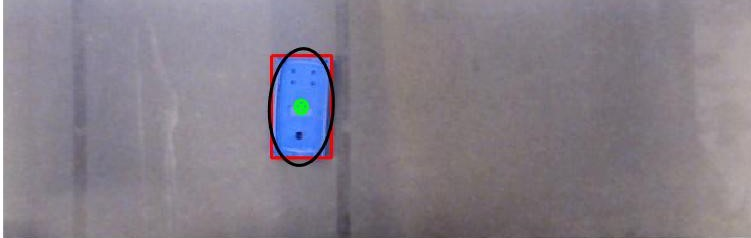
\includegraphics[width=0.8\textwidth]{elipse_hsi}
	\caption{The frame from the camera with the bounding box, centroid and equivalent ellipse plotted}
	\label{fig_ellipse}
\end{figure}\\
There is two considerations with the approach used for determination of position and orientation: firstly, for the equivalent ellipse to exist, the object needs to be rectangular, which is always the case for the housing.Secondly, the orientation is not to a specific  point on the housing, since it is simplified to a blob, this means that say the housing is rotated $180^o$ on figure \ref{fig_ellipse}, the orientation will remain the same \todo{Er dette rigtigt?}.  
\begin{figure}

\begin{tikzpicture}
\begin{axis}[
    width=0.8\textwidth,
height=0.6\textwidth,
xlabel=Frame number,
ylabel=Pixel number,
    grid=both,
grid style={line width=.1pt, draw=gray!20},
]
\addplot [
only marks,
mark size=0.6pt,
draw=blue,
] table [,y index=0]{./billeder/vision/pos.dat};
\addlegendentry{$u$ direction}
\addplot 
 [ 
only marks,
mark size=0.6pt,
color=red,
] table [y index=1]{./billeder/vision/pos.dat};
\addlegendentry{$v$ direction}
%\addplot table [y=P, x=$Q_D$]{data.dat};
%\addlegendentry{$Q_D$ series}
\end{axis}
\end{tikzpicture}
\end{figure}
